% Frequency Adaptation -- Eurographics 2027 submission draft.
% Layout approximates CGF two-column. Before submitting, move the body into the
% official egPublStyle-cgf submission template (EGauthorGuidelines-cgf-sub.tex)
% from SRMv2; this file only exists so the draft compiles here.
\documentclass[10pt,twocolumn,a4paper]{article}
\usepackage[T1]{fontenc}
\usepackage[utf8]{inputenc}
\usepackage{times}
\usepackage[margin=2cm,columnsep=6mm]{geometry}
\usepackage{graphicx,booktabs,amsmath,amssymb,xcolor}
\usepackage[hidelinks]{hyperref}
\usepackage{caption}
\captionsetup{font=small,labelfont=bf}
\setlength{\parskip}{0pt}
\usepackage[numbers,sort&compress]{natbib}
\usepackage{tikz}
\usetikzlibrary{positioning,calc}
\usepackage{pgfplots}
\pgfplotsset{compat=1.18}
\pgfplotsset{
  draft/.style={
    width=\columnwidth, height=41mm,
    axis lines=left, axis line style={line width=0.4pt},
    tick align=outside, tick style={line width=0.4pt, black},
    ymajorgrids, grid style={black!12, line width=0.3pt},
    label style={font=\scriptsize}, tick label style={font=\scriptsize},
    legend style={font=\scriptsize, draw=none, fill=none, cells={anchor=west},
                  inner sep=1pt},
    every axis plot/.append style={line width=0.7pt, mark size=1.7pt},
  }}
% generated by scripts/paper_numbers.py -- do not edit
\newcommand{\baseCannyClip}{30.34}
\newcommand{\baseCannyEdge}{0.6854}
\newcommand{\baseCannyFid}{71.92}
\newcommand{\baseCannyLpips}{0.5294}
\newcommand{\baseHedClip}{29.16}
\newcommand{\baseHedEdge}{0.5733}
\newcommand{\baseHedFid}{118.98}
\newcommand{\baseHedLpips}{0.6548}
\newcommand{\baseParams}{361,279,120}
\newcommand{\clipMainFiveZero}{29.78}
\newcommand{\clipMainOneHundred}{30.30}
\newcommand{\clipMainOneZero}{29.53}
\newcommand{\clipMainSevenZero}{29.92}
\newcommand{\clipMainThreeZero}{29.73}
\newcommand{\clipMainTwoZero}{29.47}
\newcommand{\clipMainZeroFive}{29.41}
\newcommand{\clipMainZero}{29.54}
\newcommand{\divHalfScale}{0.6061}
\newcommand{\divMainFiveZero}{0.4100}
\newcommand{\divMainOneHundred}{0.5066}
\newcommand{\divMainOneZero}{0.3414}
\newcommand{\divMainSevenZero}{0.4334}
\newcommand{\divMainThreeZero}{0.3794}
\newcommand{\divMainTwoZero}{0.3719}
\newcommand{\divMainZeroFive}{0.3126}
\newcommand{\divMainZero}{0.2994}
\newcommand{\divQuarterScale}{0.7752}
\newcommand{\divThreeQScale}{0.4171}
\newcommand{\edgeMainFiveZero}{0.6225}
\newcommand{\edgeMainOneHundred}{0.4724}
\newcommand{\edgeMainOneZero}{0.7439}
\newcommand{\edgeMainSevenZero}{0.5788}
\newcommand{\edgeMainThreeZero}{0.6878}
\newcommand{\edgeMainTwoZero}{0.7113}
\newcommand{\edgeMainZeroFive}{0.7796}
\newcommand{\edgeMainZero}{0.7776}
\newcommand{\fidEa}{56.39}
\newcommand{\fidEbase}{76.25}
\newcommand{\fidEcapb}{52.84}
\newcommand{\fidEcap}{53.17}
\newcommand{\fidEgate}{65.71}
\newcommand{\fidEres}{86.84}
\newcommand{\fidEwin}{58.51}
\newcommand{\fidHalfScale}{76.46}
\newcommand{\fidMainFiveZero}{53.97}
\newcommand{\fidMainOneHundred}{57.40}
\newcommand{\fidMainOneZero}{54.68}
\newcommand{\fidMainSevenZero}{53.69}
\newcommand{\fidMainThreeZero}{52.77}
\newcommand{\fidMainTwoZero}{53.45}
\newcommand{\fidMainZeroFive}{51.58}
\newcommand{\fidMainZero}{50.13}
\newcommand{\fidQuarterScale}{104.95}
\newcommand{\fidThreeQScale}{58.90}
\newcommand{\lpipsMainFiveZero}{0.4418}
\newcommand{\lpipsMainOneHundred}{0.5329}
\newcommand{\lpipsMainOneZero}{0.3748}
\newcommand{\lpipsMainSevenZero}{0.4625}
\newcommand{\lpipsMainThreeZero}{0.4148}
\newcommand{\lpipsMainTwoZero}{0.4003}
\newcommand{\lpipsMainZeroFive}{0.3495}
\newcommand{\lpipsMainZero}{0.3341}
\newcommand{\nTest}{3,500}
\newcommand{\nTrain}{65,100}
\newcommand{\ourParamsRatio}{55}
\newcommand{\ourParams}{6,611,469}
\newcommand{\pathAllOffThreeZero}{0.0087}
\newcommand{\pathAllOffZero}{0.0368}
\newcommand{\pathAttnOnlyThreeZero}{0.0279}
\newcommand{\pathAttnOnlyZero}{0.2112}
\newcommand{\pathBothThreeZero}{0.2347}
\newcommand{\pathBothZero}{0.6991}
\newcommand{\pathFidAllOff}{120.50}
\newcommand{\pathFidAttnOnly}{67.07}
\newcommand{\pathFidBoth}{50.13}
\newcommand{\pathFidSkipOnly}{65.12}
\newcommand{\pathSkipOnlyThreeZero}{0.1499}
\newcommand{\pathSkipOnlyZero}{0.5370}
\newcommand{\scEaOneZero}{0.0772}
\newcommand{\scEaThreeZero}{0.0314}
\newcommand{\scEaZeroFive}{0.1485}
\newcommand{\scEbaseOneZero}{0.0147}
\newcommand{\scEbaseThreeZero}{0.0172}
\newcommand{\scEbaseZeroFive}{0.0234}
\newcommand{\scEcapOneZero}{0.1882}
\newcommand{\scEcapThreeZero}{0.0739}
\newcommand{\scEcapZeroFive}{0.2826}
\newcommand{\scEcapbOneZero}{0.2158}
\newcommand{\scEcapbThreeZero}{0.0816}
\newcommand{\scEcapbZeroFive}{0.2986}
\newcommand{\scEgateOneZero}{0.0177}
\newcommand{\scEgateThreeZero}{0.0198}
\newcommand{\scEgateZeroFive}{0.0303}
\newcommand{\scEresOneZero}{0.0171}
\newcommand{\scEresThreeZero}{0.0291}
\newcommand{\scEresZeroFive}{0.0271}
\newcommand{\scEwinOneZero}{0.0218}
\newcommand{\scEwinThreeZero}{0.0255}
\newcommand{\scEwinZeroFive}{0.0359}
\newcommand{\scHalfScale}{0.2146}
\newcommand{\scMainFiveZero}{0.1259}
\newcommand{\scMainOneHundred}{0.0010}
\newcommand{\scMainOneZero}{0.6211}
\newcommand{\scMainSevenZero}{0.1110}
\newcommand{\scMainThreeZero}{0.2347}
\newcommand{\scMainTwoZero}{0.4019}
\newcommand{\scMainZeroFive}{0.7469}
\newcommand{\scMainZero}{0.6991}
\newcommand{\scQuarterScale}{0.0408}
\newcommand{\scThreeQScale}{0.4893}
\newcommand{\seedMeanFiveZero}{0.1304}
\newcommand{\seedMeanOneZero}{0.6245}
\newcommand{\seedMeanSevenZero}{0.1261}
\newcommand{\seedMeanThreeZero}{0.2318}
\newcommand{\seedMeanTwoZero}{0.4036}
\newcommand{\seedMeanZeroFive}{0.7479}
\newcommand{\seedStdFiveZero}{0.0093}
\newcommand{\seedStdOneZero}{0.0059}
\newcommand{\seedStdSevenZero}{0.0186}
\newcommand{\seedStdThreeZero}{0.0106}
\newcommand{\seedStdTwoZero}{0.0098}
\newcommand{\seedStdZeroFive}{0.0015}
\newcommand{\semMainFiveZero}{0.0047}
\newcommand{\semMainOneHundred}{0.0006}
\newcommand{\semMainOneZero}{0.0035}
\newcommand{\semMainSevenZero}{0.0047}
\newcommand{\semMainThreeZero}{0.0041}
\newcommand{\semMainTwoZero}{0.0037}
\newcommand{\semMainZeroFive}{0.0030}
\newcommand{\semMainZero}{0.0070}
\newcommand{\sketchFaceClip}{23.43}
\newcommand{\sketchFaceN}{40}
\newcommand{\sketchFaceSC}{0.5484}
\newcommand{\sketchSceneClip}{22.63}
\newcommand{\sketchSceneFid}{285.91}
\newcommand{\sketchSceneN}{500}
\newcommand{\sketchSceneSC}{0.1714}
\newcommand{\specFiveZero}{0.1211}
\newcommand{\specOneZero}{0.7049}
\newcommand{\specSevenZero}{0.1287}
\newcommand{\specThreeZero}{0.1214}
\newcommand{\specZFiveZero}{-0.7}
\newcommand{\specZOneZero}{+17.5}
\newcommand{\specZSevenZero}{+2.6}
\newcommand{\specZThreeZero}{-19.0}
\newcommand{\vaeNativeOneZero}{0.8562}
\newcommand{\vaeNativeSevenZero}{0.0700}
\newcommand{\vaeNativeThreeZero}{0.5773}
\newcommand{\vaeUpOneZero}{0.9599}
\newcommand{\vaeUpSevenZero}{0.1321}
\newcommand{\vaeUpThreeZero}{0.7978}


\title{\vspace{-1.5em}\bfseries A Frequency Dial for Structure-Conditioned Diffusion}
\author{Anonymous submission}
\date{}

\begin{document}
\maketitle

\begin{abstract}
\noindent
A structure-conditioned diffusion adapter is trained for one operating point.
Canny edges, a depth map, a sketch: each fixes how tightly the output must
follow the condition, and moving that trade-off means training again. We train
a single adapter on conditions whose information content is randomised --- a
high-pass filter whose cutoff $r$ is drawn per sample --- and read $r$ back at
test time as a dial. On FFHQ-512, structure consistency runs from
\scMainZeroFive{} at $r{=}0.05$ to \scMainSevenZero{} at $r{=}0.7$ while
sample diversity rises from \divMainZeroFive{} to \divMainSevenZero{}, and FID
stays between \fidMainThreeZero{} and \fidMainOneHundred{} across the whole
range. Turning the adapter's strength down instead reaches the same structure
consistency at a cost of up to \fidQuarterScale{} FID against \fidMainFiveZero{}
for the frequency dial, so the two knobs are not interchangeable.

Two findings came out of building it. The frozen SD VAE destroys a high-pass
condition before any adapter can read it: only \vaeNativeThreeZero{} of the
condition survives an encode--decode round trip at $r{=}0.3$ and
\vaeNativeSevenZero{} at $r{=}0.7$. And placement dominates capacity ---
residuals on the decoder skip connections carry \pathSkipOnlyZero{} of the
structure signal against \pathAttnOnlyZero{} for cross-attention injection,
while quadrupling adapter width buys far less. The adapter trains
\ourParams{} parameters, \ourParamsRatio{}$\times$ fewer than ControlNet.
\end{abstract}

\section{Introduction}

ControlNet~\cite{zhang2023adding} and its successors~\cite{mou2023adapter,zhao2023controlnet,qin2023unicontrol,li2024controlnet} solved conditional control and then froze it.
An adapter trained on Canny edges follows Canny edges; one trained on depth
follows depth. The strength of that following is a property of the trained
weights, so an artist who wants the same sketch honoured more loosely has to
pick a different checkpoint or accept whatever the one they have was trained to
do.

We change what the condition is rather than how hard the model listens to it.
The condition is the image after a radial high-pass filter with normalised
cutoff $r$. At $r{=}0$ the model receives the grayscale image and the task is
colourisation. As $r$ grows the filter removes more of the spectrum, until at
$r{=}1$ almost nothing is left: measured on FFHQ, a cutoff of $0.05$ already
discards 97.5\,\% of the spectral energy. Training draws $r$ per sample, so one
set of weights sees the whole range, and $r$ becomes an inference-time
parameter.

Our contributions are:

\begin{itemize}\itemsep2pt
\item A control dial. One adapter spans structure consistency
      \scMainZeroFive{} to \scMainSevenZero{} with FID flat between
      \fidMainThreeZero{} and \fidMainOneHundred{} (Sec.~\ref{sec:dial}).
\item Evidence that the dial is not a rescaled version of adapter strength.
      At matched structure consistency the strength knob costs
      \fidQuarterScale{} FID where the frequency knob costs
      \fidMainFiveZero{} (Sec.~\ref{sec:strength}).
\item A measurement of how much of a high-pass condition survives the frozen
      VAE, which explains why latent-space conditioning fails for sparse
      structure (Sec.~\ref{sec:vae}).
\item A controlled comparison of injection sites showing that placement
      matters more than adapter capacity or receptive field
      (Sec.~\ref{sec:where}).
\end{itemize}

\section{Related work}

\paragraph{Conditional control.} Text-to-image diffusion
\cite{ho2020denoising,song2020denoising,rombach2021high,nichol2021glide,saharia2022photorealistic}
became spatially controllable with ControlNet~\cite{zhang2023adding}, which
duplicates the encoder and injects residuals through zero convolutions.
T2I-Adapter~\cite{mou2023adapter} does the same job with a small feature
extractor, IP-Adapter~\cite{ye2023adapter} adds decoupled cross-attention for
image prompts, and GLIGEN~\cite{li2023gligen} grounds generation on boxes.
Uni-ControlNet~\cite{zhao2023controlnet} and UniControl~\cite{qin2023unicontrol}
fold many condition types into one model, and
ControlNet++~\cite{li2024controlnet} closes a consistency loop on the produced
image. Each of these fixes the condition type and, with it, how tightly the
output must follow: the operating point is a property of the trained weights.
Our cutoff moves that point at inference on one set of weights.

\paragraph{Efficient control on transformer backbones.} As backbones moved from
UNets to diffusion transformers~\cite{peebles2022scalable,esser2024scaling},
control moved from duplicated encoders to lightweight modules.
ControlNeXt~\cite{peng2024controlnext} removes the parallel branch,
OminiControl~\cite{tan2024ominicontrol} reuses the backbone itself as the
condition processor, and EasyControl~\cite{zhang2025easycontrol} and
NanoControl~\cite{liu2025nanocontrol} inject conditions through
LoRA-style~\cite{hu2021lora} modules at a small fraction of the parameter cost.
Recent work also examines where conditions should enter:
Laytrol~\cite{huang2025laytrol} on preserving pretrained knowledge under layout
control, PixelControl~\cite{lin2026pixelcontrol} on condition fidelity, and
\citet{zhou2026rethinking} on removing redundant attention in multi-condition
DiTs. Our injection-site comparison (Sec.~\ref{sec:where}) reaches a compatible
conclusion on a UNet backbone: placement dominates capacity.

\paragraph{Frequency in diffusion.} Frequency decomposition appears in diffusion
mostly as an intervention on the model's own signals rather than on its
condition. FreeU~\cite{si2023freeu} rebalances skip and backbone features
spectrally at no training cost, FreSca~\cite{huang2025fresca} scales frequency
bands of the noise prediction and, like us, uses an energy-based cutoff,
DeCo~\cite{ma2025deco} decouples frequencies in pixel-space diffusion, and
FeRA~\cite{yin2025fera} routes adaptation by frequency energy.
FOCUS~\cite{tjio2025focus} conditions the reverse process on learned frequency
priors for test-time adaptation. Closest to us in spirit,
\citet{prasain2026beyond} condition on wavelet bands instead of edge maps for
map-to-satellite synthesis. What none of these do is randomise the condition's
bandwidth during training so that the band becomes a control at inference,
which is the mechanism we study.

\paragraph{Structure preservation.} StructDiff~\cite{he2026structdiff} targets
structure-preserving spatially controllable generation, and sketch-conditioned
pipelines have long used edge maps as the structural carrier. Our condition is
a continuum rather than a fixed extractor, which is what makes a dial possible.

\paragraph{Training and evaluation.} We train with classifier-free
guidance~\cite{ho2022classifier} dropout and Min-SNR loss
weighting~\cite{hang2023efficient}, and evaluate with FID~\cite{heusel2017gans}
under the clean-FID protocol~\cite{parmar2021aliased},
LPIPS~\cite{zhang2018unreasonable} and CLIP score~\cite{radford2021learning} on
FFHQ~\cite{karras2018style} with BLIP~\cite{li2022blip} captions. SDXL and
SD3~\cite{podell2023sdxl,esser2024scaling} are the natural next backbones.

\section{Method}

\paragraph{Condition.} Given an image $x$, we convert to grayscale, take the
2D FFT, zero every frequency inside a disc of radius $r \cdot \min(H,W)/2$,
invert, and min--max normalise to $[0,1]$. The normalisation is deliberate: it
removes the absolute scale of the filter response, so the model has to infer
structure density from spatial statistics. That is what lets a hand drawing,
which has no $r$, be used at test time.

% What the dial actually does, from radial_mask_numpy / high_pass_numpy in the
% repository, so the picture and the method cannot diverge.
\begin{figure*}[t]
\centering

\includegraphics[width=\textwidth]{figures/mask}
\caption{The dial, from the frequency side. Columns are
$r = 0,\,0.05,\,0.1,\,0.2,\,0.3,\,0.5,\,0.7,\,1.0$. \textbf{Row 1:} the radial
mask; black is removed. \textbf{Row 2:} the log-magnitude spectrum after
masking, with the hole growing outward. \textbf{Row 3:} the resulting
condition, exactly as the model receives it. \textbf{Row 4:} the same data
displayed at $\pm2\sigma$ so that the residual content is visible.
Above $r{\approx}0.2$ the condition looks like flat grey --- its standard
deviation falls from 0.196 at $r{=}0$ to 0.041 at $r{=}1$ --- yet the face
outline survives in row 4, and the model still reaches
SC \scMainTwoZero{} at $r{=}0.2$. Low contrast is not the same as no
information, which is what the per-image normalisation forces the model to
learn.}
\label{fig:mask}
\end{figure*}


\paragraph{Condition encoder.} A strided convolutional stem reads the condition
image directly at $512^2$ and reduces it $8\times$. We do not encode the
condition with the frozen VAE; Sec.~\ref{sec:vae} shows why.

\paragraph{Injection.} Encoder features enter the UNet in two places. Zero-initialised
$1{\times}1$ heads produce one residual per decoder skip tensor and one for the
mid block, added through the UNet's existing ControlNet interface. In parallel,
each cross-attention site attends over a $3{\times}3$ window of the condition
features, gated by a zero-initialised per-channel vector. Both paths start as
exact no-ops: with them switched off the network reproduces stock
Stable Diffusion~1.5~\cite{rombach2021high} bit for bit, which we assert before every training run.

% Architecture schematic. Drafted, not illustrated: one stroke weight for data
% flow, a heavier one for trained parts, flat tint for the frozen backbone,
% square corners, no shadows. The U places the skip tensors where the residuals
% actually land.
\begin{figure*}[t]
\centering
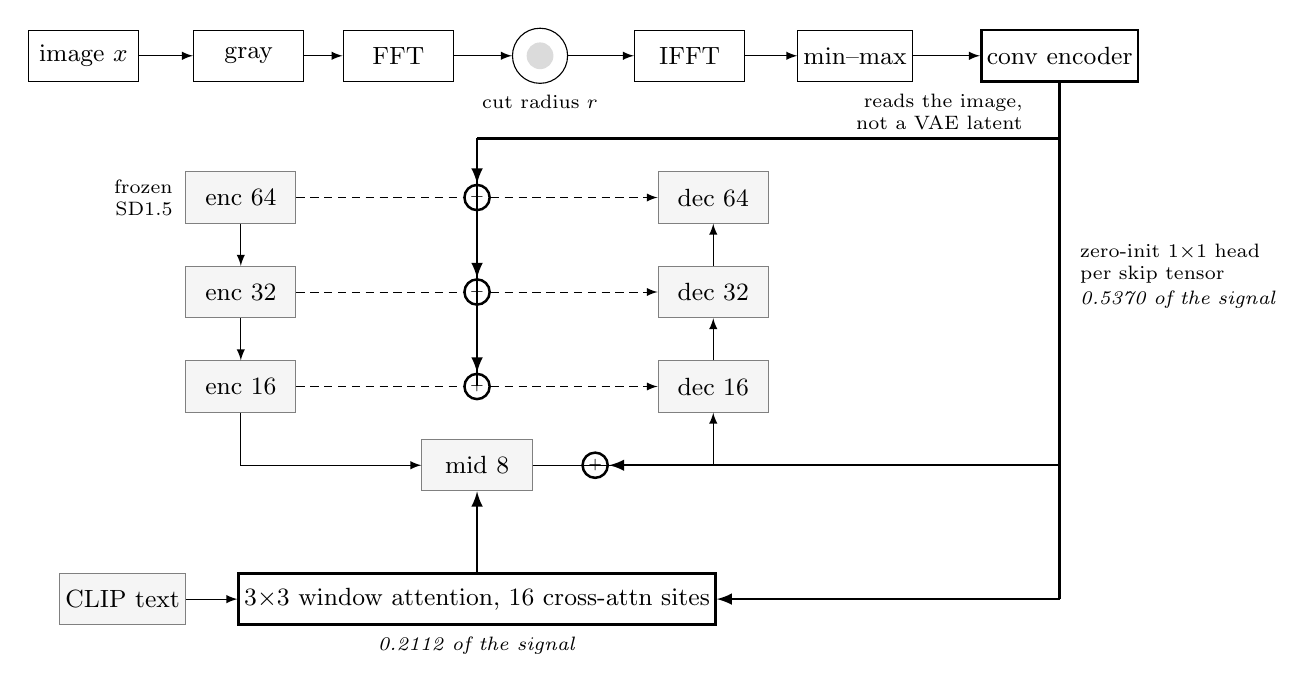
\begin{tikzpicture}[
  font=\small, >=latex, line width=0.4pt,
  blk/.style   ={draw, minimum height=6.5mm, minimum width=14mm, inner xsep=2pt, align=center},
  frozen/.style={blk, fill=black!4, draw=black!50},
  train/.style ={blk, line width=0.9pt},
  lbl/.style   ={font=\scriptsize, inner sep=1.5pt},
  flow/.style  ={->, line width=0.4pt},
  inj/.style   ={->, line width=0.9pt},
  skip/.style  ={densely dashed, line width=0.35pt},
  sum/.style   ={draw, circle, inner sep=0pt, minimum size=3.2mm, line width=0.9pt},
]

% ================= condition construction =================
\node[blk] (img)  at (0,0.9) {image $x$};
\node[blk] (gray) at (2.1,0.9) {gray};
\node[blk] (fft)  at (4.0,0.9) {FFT};
\node[draw, circle, minimum size=7mm, inner sep=0pt] (mask) at (5.8,0.9) {};
\fill[black!14] (mask.center) circle (1.7mm);
\node[blk] (ifft) at (7.7,0.9) {IFFT};
\node[blk] (norm) at (9.8,0.9) {min--max};
\node[train] (enc) at (12.4,0.9) {conv encoder};
\foreach \a/\b in {img/gray, gray/fft, fft/mask, mask/ifft, ifft/norm, norm/enc}
  \draw[flow] (\a) -- (\b);
\node[lbl, below=0.8mm of mask, align=center] {cut radius $r$};
\node[lbl, below left=0.8mm and -6mm of enc, align=right] {reads the image,\\not a VAE latent};

% ================= frozen UNet, drawn as a U =================
\node[frozen] (e64) at (2.0,-0.9) {enc 64};
\node[frozen] (e32) at (2.0,-2.1) {enc 32};
\node[frozen] (e16) at (2.0,-3.3) {enc 16};
\node[frozen] (mid) at (5.0,-4.3) {mid 8};
\node[frozen] (d16) at (8.0,-3.3) {dec 16};
\node[frozen] (d32) at (8.0,-2.1) {dec 32};
\node[frozen] (d64) at (8.0,-0.9) {dec 64};
\foreach \a/\b in {e64/e32, e32/e16} \draw[flow] (\a) -- (\b);
\draw[flow] (e16) |- (mid);
\draw[flow] (mid) -| (d16);
\foreach \a/\b in {d16/d32, d32/d64} \draw[flow] (\a) -- (\b);
\node[lbl, left=1mm of e64, align=right] {frozen\\SD1.5};

% skip tensors, with the summing junction the residual lands on
\foreach \lv/\y in {64/-0.9, 32/-2.1, 16/-3.3}{
  \node[sum] (s\lv) at (5.0,\y) {\tiny$+$};
  \draw[skip] (e\lv) -- (s\lv);
  \draw[skip, ->] (s\lv) -- (d\lv);
}
\node[sum] (smid) at (6.5,-4.3) {\tiny$+$};

% ================= injection path 1: skip residuals =================
% one trunk down the right margin, tapped where nothing else runs
\draw[line width=0.9pt] (enc.south) -- (12.4,-6.0);
\draw[line width=0.9pt] (12.4,-0.15) -- (5.0,-0.15);
\foreach \n in {s64,s32,s16}{ \draw[inj] (5.0,-0.15) -- (\n.north); }
\draw[line width=0.9pt] (5.0,-0.15) -- (5.0,-3.3);
\draw[inj] (12.4,-4.3) -- (smid.east);
\node[lbl, right=1mm] at (12.5,-1.9) {\begin{minipage}{25mm}\raggedright
  zero-init $1{\times}1$ head per skip tensor\\[1pt]
  \emph{\pathSkipOnlyZero{} of the signal}\end{minipage}};

% ================= injection path 2: window attention =================
\node[train, minimum width=42mm] (attn) at (5.0,-6.0)
  {$3{\times}3$ window attention, 16 cross-attn sites};
\draw[inj] (12.4,-6.0) -- (attn.east);
\draw[inj] (attn.north) -- (mid.south);
\node[lbl, below=0.8mm of attn] {\emph{\pathAttnOnlyZero{} of the signal}};

\node[frozen, minimum width=16mm] (clip) at (0.5,-6.0) {CLIP text};
\draw[flow] (clip) -- (attn.west);

\end{tikzpicture}
\caption{Condition construction (top) and the two injection paths. A disc of
radius $r$ is masked out of the spectrum; a trainable convolutional encoder
reads the result at full resolution. Heavy strokes are trained
(\ourParams{} parameters), tinted blocks are frozen, and $\oplus$ marks where a
zero-initialised residual is added to a skip tensor. With both paths off the
network reproduces stock SD1.5 exactly. The skip path carries most of the
structure signal; Sec.~\ref{sec:where} measures the split.}
\label{fig:arch}
\end{figure*}


\paragraph{Training.} SD1.5~\cite{rombach2021high} stays frozen. We train \ourParams{} parameters on
\nTrain{} FFHQ-512~\cite{karras2018style} images with BLIP~\cite{li2022blip} captions, batch 32, bf16, 12 epochs, on one
H200. $r$ is drawn uniformly from $[0,1]$ per sample.

\section{Experiments}

We evaluate on \nTest{} held-out images, 50 sampler steps, CFG 7.5, seed 2026.
We report FID~\cite{heusel2017gans} with the clean-FID protocol~\cite{parmar2021aliased},
LPIPS~\cite{zhang2018unreasonable} and CLIP score~\cite{radford2021learning}.
Structure consistency (SC) re-extracts the condition from the generated image
at the same cutoff and correlates it with the condition the model was given.
Feeding the ground truth back gives exactly 1.000 at every $r$; an unrelated
face gives 0.122 at $r{=}0$ and ${\approx}{-}0.02$ above it.

\begin{figure*}[t]
\centering

\includegraphics[width=\textwidth]{figures/dial}
\caption{One seed, one caption, $r$ swept. Columns: reference, then
$r = 0,\,0.05,\,0.1,\,0.3,\,0.5,\,0.7,\,1.0$. The background crowd thins out,
the eyewear drifts from the reference frame, and the clothing colour detaches,
while identity and pose survive. The reference is never shown to the model.}
\label{fig:dial}
\end{figure*}

\subsection{The dial}
\label{sec:dial}

Table~\ref{tab:main} gives the operating curve. Structure consistency falls
monotonically from $r{=}0.05$ and sample diversity rises monotonically, which
is the trade-off the dial is supposed to expose. FID stays between
\fidMainZero{} and \fidMainOneHundred{} across the entire sweep, so the range is
usable end to end rather than degrading into noise.

Figure~\ref{fig:dial} holds the seed and the caption fixed and varies only $r$.
Figure~\ref{fig:curve} plots the curve and, below it, both dials in the same
structure-consistency/FID plane.

% Operating curves. Both panels read curve.dat / scale.dat, which
% scripts/paper_numbers.py writes out of results/, so a plotted point cannot
% drift from the run that produced it. Drafted to match the text: hairline
% axes, no boxes, no fills, marks a reader can count.
\begin{figure}[t]
\centering
\begin{tikzpicture}
\begin{axis}[draft, xlabel={cutoff $r$}, ylabel={SC / diversity (LPIPS)},
             xmin=-0.03, xmax=1.03, ymin=0, ymax=0.8,
             legend pos=north east]
  \addplot[mark=square*, black] table[x=r, y=sc] {curve.dat};
  \addlegendentry{structure consistency}
  \addplot[mark=o, black, densely dashed] table[x=r, y=div] {curve.dat};
  \addlegendentry{sample diversity}
\end{axis}
\end{tikzpicture}

\vspace{2mm}

\begin{tikzpicture}
\begin{axis}[draft, height=38mm,
             xlabel={structure consistency}, ylabel={FID},
             xmin=-0.03, xmax=0.8, ymin=45, ymax=112,
             legend columns=2,
             legend style={at={(0.5,-0.42)}, anchor=north}]
  \addplot[mark=square*, black, restrict expr to domain={\thisrow{r}}{0.04:0.31}] table[x=sc, y=fid] {curve.dat};
  \addlegendentry{cutoff, own instrument}
  \addplot[only marks, mark=square, black!45, y filter/.expression={(\thisrow{r}>0.04 && \thisrow{r}<0.31) ? nan : y}] table[x=sc, y=fid] {curve.dat};
  \addlegendentry{cutoff outside $[0.05, 0.3]$}
  \addplot[mark=diamond*, black, densely dotted] coordinates {(\fixInstZeroFive,\fidMainZeroFive) (\fixInstOneZero,\fidMainOneZero) (\fixInstTwoZero,\fidMainTwoZero) (\fixInstThreeZero,\fidMainThreeZero)};
  \addlegendentry{cutoff, instrument $r_m{=}0.1$}
  \addplot[mark=o, black, densely dashed] table[x=sc, y=fid] {scale.dat};
  \addlegendentry{randomised-$r$ at $r{=}0.1$, scaled}
  \addplot[mark=triangle, black!55, dotted] coordinates {(\sscSCQuarter,\sscFidQuarter) (\sscSCHalf,\sscFidHalf) (\sscSCThreeQ,\sscFidThreeQ) (\sscSCOne,\sscFidOne)};
  \addlegendentry{fixed-$r{=}0.1$ adapter, scaled}
\end{axis}
\end{tikzpicture}
\caption{\textbf{Top:} structure consistency and sample diversity against the
cutoff (values of Table~\ref{tab:main}, which gives SEM and seed sd).
\textbf{Bottom:} FID against structure consistency, one FID estimate per point.
Filled squares: the cutoff sweep scored at its own cutoff on $r \in [0.05, 0.3]$;
open grey squares: the same sweep outside that range. Diamonds: the same
generations re-scored with the instrument fixed at $r_m{=}0.1$. Circles and
triangles: the randomised-$r$ and fixed-$r{=}0.1$ adapters scaled at
$r{=}0.1$, which already use $r_m{=}0.1$. On that one instrument the cutoff
$r{=}0.3$ reaches \fixInstThreeZero{} at FID \fidMainThreeZero{}, while scale
0.50 reaches \fixInstHalfScale{} at FID \fidHalfScale{}. Both panels are
plotted directly from the evaluation outputs.}
\label{fig:curve}
\end{figure}


\begin{table}[t]\centering\small
\begin{tabular}{lrrrrr}
\toprule
$r$ & SC & Diversity & LPIPS & CLIP & FID \\
\midrule
0.00 & \scMainZero      & \divMainZero      & \lpipsMainZero      & \clipMainZero      & \fidMainZero \\
0.05 & \scMainZeroFive  & \divMainZeroFive  & \lpipsMainZeroFive  & \clipMainZeroFive  & \fidMainZeroFive \\
0.10 & \scMainOneZero   & \divMainOneZero   & \lpipsMainOneZero   & \clipMainOneZero   & \fidMainOneZero \\
0.20 & \scMainTwoZero   & \divMainTwoZero   & \lpipsMainTwoZero   & \clipMainTwoZero   & \fidMainTwoZero \\
0.30 & \scMainThreeZero & \divMainThreeZero & \lpipsMainThreeZero & \clipMainThreeZero & \fidMainThreeZero \\
0.50 & \scMainFiveZero  & \divMainFiveZero  & \lpipsMainFiveZero  & \clipMainFiveZero  & \fidMainFiveZero \\
0.70 & \scMainSevenZero & \divMainSevenZero & \lpipsMainSevenZero & \clipMainSevenZero & \fidMainSevenZero \\
1.00 & \scMainOneHundred& \divMainOneHundred& \lpipsMainOneHundred& \clipMainOneHundred& \fidMainOneHundred \\
\bottomrule
\end{tabular}
\caption{Operating curve, \nTest{}-image test split, 500 sampled.}
\label{tab:main}
\end{table}

Across seeds 2026, 2027 and 2028 the curve is stable: SC at $r{=}0.05$ is
\seedMeanZeroFive{}\,$\pm$\,\seedStdZeroFive{} and at $r{=}0.3$ it is
\seedMeanThreeZero{}\,$\pm$\,\seedStdThreeZero{}.

\subsection{Strength is not the same knob}
\label{sec:strength}

An obvious alternative is to train on one cutoff and scale the adapter's
contribution at inference. We tested it on the same checkpoint, holding
$r{=}0.1$ and scaling both injection paths.

\begin{table}[h]\centering\small
\begin{tabular}{lrrr}
\toprule
Setting & SC & Diversity & FID \\
\midrule
scale 0.25          & \scQuarterScale & \divQuarterScale & \fidQuarterScale \\
scale 0.50          & \scHalfScale    & \divHalfScale    & \fidHalfScale \\
scale 0.75          & \scThreeQScale  & \divThreeQScale  & \fidThreeQScale \\
\midrule
$r{=}0.3$ (ours)    & \scMainThreeZero & \divMainThreeZero & \fidMainThreeZero \\
$r{=}0.5$ (ours)    & \scMainFiveZero  & \divMainFiveZero  & \fidMainFiveZero \\
\bottomrule
\end{tabular}
\caption{Strength dial against frequency dial. Reading across matched SC:
scale 0.50 reaches \scHalfScale{} at FID \fidHalfScale{}, while $r{=}0.3$
reaches \scMainThreeZero{} at FID \fidMainThreeZero{}.}
\label{tab:strength}
\end{table}

Weakening the adapter degrades the image; narrowing the condition's bandwidth
does not. The frequency parameterisation is what makes the trade-off traversable.

\subsection{The VAE eats the condition}
\label{sec:vae}

% How much of the condition survives the frozen VAE. Plotted from vae.dat,
% written by scripts out of results/. Same drafting as the other plots.
\begin{figure}[t]
\centering
\begin{tikzpicture}
\begin{axis}[draft, height=42mm,
  xlabel={cutoff $r$}, ylabel={correlation after round trip},
  xmin=-0.03, xmax=1.03, ymin=0, ymax=1.05,
  legend pos=north east]
  \addplot[mark=square*, black] table[x=r, y=native] {vae.dat};
  \addlegendentry{condition built at 512}
  \addplot[mark=o, black, densely dashed] table[x=r, y=up256] {vae.dat};
  \addlegendentry{built at 256, upsampled}
\end{axis}
\end{tikzpicture}
\caption{Correlation between the condition fed to the autoencoder and the same
condition re-extracted after an encode--decode round trip, the first 24
FFHQ-512 images in file order, which are not the test split. Above
$r{\approx}0.5$ the condition is effectively gone. Building the condition at 256
and upsampling puts the
structure at lower absolute frequency and preserves far more, which is why
comparisons against older pipelines need the source resolution stated.}
\label{fig:vae}
\end{figure}


Encoding the condition with the frozen SD VAE, as an IP-Adapter-style~\cite{ye2023adapter} design
would, loses most of it. Figure~\ref{fig:vae} plots it. Passing the condition through encode--decode and
re-measuring leaves \vaeNativeOneZero{} at $r{=}0.1$, \vaeNativeThreeZero{} at
$r{=}0.3$ and \vaeNativeSevenZero{} at $r{=}0.7$. An adapter reading that latent
cannot recover information the autoencoder has already discarded. Building the
condition at 256 and upsampling moves the structure to lower absolute frequency
and preserves far more (\vaeUpThreeZero{} at $r{=}0.3$), which is a data-pipeline
artefact worth knowing about when comparing against older setups.

\subsection{Where to inject}
\label{sec:where}

% Injection-path decomposition. Bars are drawn from paths.dat; the dashed rule
% marks the all-off control, so every bar is read against what the frozen
% backbone alone achieves.
\begin{figure}[t]
\centering
\begin{tikzpicture}
\begin{axis}[draft, height=44mm, width=0.95\columnwidth,
  ybar, bar width=7pt,
  xlabel={}, ylabel={structure consistency},
  symbolic x coords={both,skip,attn,off},
  xtick=data,
  xticklabels={both paths, skip only\\(test time), attn only\\(test time), both off},
  x tick label style={font=\scriptsize, align=center},
  ymin=0, ymax=0.78,
  legend pos=north east,
  enlarge x limits=0.16,
  every axis plot/.append style={line width=0.4pt}]
  \addplot[fill=black!72, draw=black, area legend] table[x=label, y=sc0] {paths.dat};
  \addlegendentry{$r{=}0$}
  \addplot[fill=black!22, draw=black, area legend] table[x=label, y=sc3] {paths.dat};
  \addlegendentry{$r{=}0.3$}
  \draw[densely dashed, black!55, line width=0.4pt]
    (axis cs:both,\pathAllOffZero) -- (axis cs:off,\pathAllOffZero);
  \addlegendimage{line legend, densely dashed, black!55, line width=0.4pt}
  \addlegendentry{both off, $r{=}0$}
\end{axis}
\end{tikzpicture}
\caption{Both injection paths on, then each alone, then neither. The skip
residuals carry most of the structure signal; cross-attention alone recovers
little of it, and with both off the model falls to the frozen backbone
(FID \pathFidAllOff{} against \pathFidBoth{} with both paths on; skip only
\pathFidSkipOnly{}, attention only \pathFidAttnOnly{}). The dashed line is the
both-off control at $r{=}0$. Paths are switched off at test time on the trained
main model; the separately trained skip-only model is in
Table~\ref{tab:skiponly}. At $r{=}0$ the single-path gains over the control
roughly add up to the both-paths gain; at $r{=}0.3$ the both-paths gain over
the control exceeds the sum of the single-path gains.}
% <<AUTHOR-INPUT A39: (선택) r=0.3에서 두 경로가 서로 무엇을 보완한다고 보는지 한 문장 -- 넣는다면 §5.2 본문에. 쓰지 않으면 이 줄을 지운다>>
\label{fig:paths}
\end{figure}


Starting from the same encoder and training schedule, we varied one field at a
time (Table~\ref{tab:where}). Skip-connection residuals dominate. Figure~\ref{fig:paths} decomposes them. Ablating them
away and keeping only cross-attention drops SC at $r{=}0$ from
\pathBothZero{} to \pathAttnOnlyZero{}; keeping only the skip path retains
\pathSkipOnlyZero{}. With both paths off the model collapses to
\pathAllOffZero{} SC and FID \pathFidAllOff{}, which is the control that says
the adapter is doing the work.

Capacity helps much less: widening the projection to a 128-channel stem raises
SC at $r{=}0.05$ from \scEaZeroFive{} to \scEcapZeroFive{}, and doubling again
to 256 reaches only \scEcapbZeroFive{}. A $7{\times}7$ attention window is worse
than $3{\times}3$ (\scEwinZeroFive{}).

\begin{table}[h]\centering\small
\begin{tabular}{lrrr}
\toprule
Variant & SC $r{=}0.05$ & SC $r{=}0.1$ & FID $r{=}0.1$ \\
\midrule
VAE condition, attn only    & \scEbaseZeroFive & \scEbaseOneZero & \fidEbase \\
\quad + zero-init gate      & \scEgateZeroFive & \scEgateOneZero & \fidEgate \\
Conv condition encoder      & \scEaZeroFive    & \scEaOneZero    & \fidEa \\
\quad + 128-ch stem         & \scEcapZeroFive  & \scEcapOneZero  & \fidEcap \\
\quad + 256-ch stem         & \scEcapbZeroFive & \scEcapbOneZero & \fidEcapb \\
\quad + $7{\times}7$ window & \scEwinZeroFive  & \scEwinOneZero  & \fidEwin \\
\quad + skip residuals      & \scMainZeroFive  & \scMainOneZero  & \fidMainOneZero \\
\bottomrule
\end{tabular}
\caption{One field changed per row against the row above it.}
\label{tab:where}
\end{table}

\subsection{Against per-cutoff specialists}

We trained four adapters at fixed $r$ and compared each against the single
randomised-$r$ model at its own cutoff. The result is mixed: the specialist
wins at $r{=}0.1$ (\specOneZero{} against \scMainOneZero{},
$z{=}\specZOneZero{}$) and marginally at $r{=}0.7$ ($z{=}\specZSevenZero{}$),
the single model wins at $r{=}0.3$ (\scMainThreeZero{} against \specThreeZero{},
$z{=}\specZThreeZero{}$), and $r{=}0.5$ is a tie ($z{=}\specZFiveZero{}$).

One model therefore does not dominate four. What it does instead is give a dial
the specialists cannot: a model trained at $r{=}0.1$ has never seen $r{=}0.3$,
so its curve is a single point.

\subsection{Baselines}

Against pretrained ControlNet~\cite{zhang2023adding} on its own condition, over the same test images
and captions: ControlNet-Canny reaches Edge-F1 \baseCannyEdge{}, LPIPS
\baseCannyLpips{}, FID \baseCannyFid{} with \baseParams{} trainable parameters;
ControlNet-HED reaches \baseHedEdge{} / \baseHedLpips{} / \baseHedFid{}. At
$r{=}0.1$ our adapter reaches Edge-F1 \edgeMainOneZero{}, LPIPS
\lpipsMainOneZero{} and FID \fidMainOneZero{} with \ourParams{} parameters.
The conditions differ --- Canny edges against a frequency band --- so this is a
comparison of operating points, not a like-for-like control.

\subsection{Hand-drawn sketches}
\begin{figure}[t]
\centering
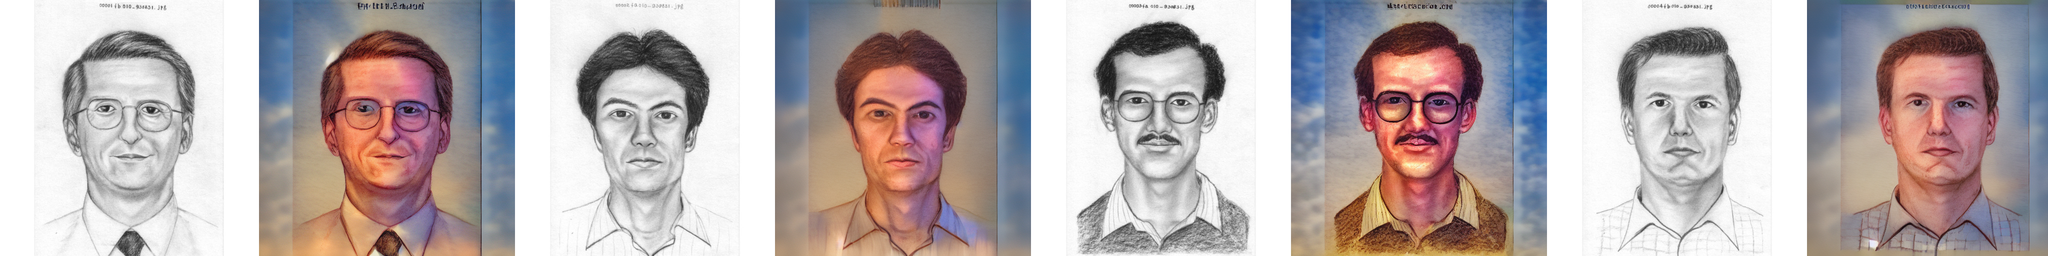
\includegraphics[width=\columnwidth]{figures/sketch}
\caption{Hand-drawn face sketches (odd columns) and what the model makes of
them (even columns), zero-shot. The drawings carry no cutoff; the model has to
read structure density off the drawing itself, which the per-image min--max
normalisation of the condition is what permits.}
\label{fig:sketch}
\end{figure}


Figure~\ref{fig:sketch} shows the transfer. On \sketchFaceN{} real face
drawings the model was never trained on, structure
consistency against the input drawing is \sketchFaceSC{} and CLIP score is
\sketchFaceClip{}. FID is not reported: \sketchFaceN{} images is too few for a
stable estimate, and our evaluator refuses rather than print one.

\section{Limitations}

The useful range is roughly $r \in [0, 0.3]$. Above it the condition retains
little energy --- 0.0014 of the spectrum at $r{=}0.5$ --- and structure
consistency becomes hard to interpret, since two nearly empty signals correlate
near zero whatever the model does.

Everything here is one domain (FFHQ faces) and one backbone (SD1.5). Current
structure-control work has moved to DiT backbones~\cite{peebles2022scalable,esser2024scaling}, where
LoRA-style~\cite{hu2021lora} adapters~\cite{tan2024ominicontrol,zhang2025easycontrol,liu2025nanocontrol}
report control at a fraction of our parameter count; our efficiency numbers
should be read against ControlNet, not against that line.

The specialist comparison is honest but unflattering at $r{=}0.1$, and we have
not run a user study.

\section{Conclusion}

Randomising the bandwidth of a structure condition during training turns the
cutoff into an inference-time control, and that control is not reproducible by
scaling the adapter down. Getting there required fixing where the condition
enters the network and keeping it out of the frozen autoencoder; both of those
findings transfer to other conditioning designs regardless of what the dial is
used for.

\bibliographystyle{plainnat}
\bibliography{refs}

\end{document}
